	\chapter{Detalles de implementaci\'on}

\section{Introducci\'on}

En el siguiente cap\'itulo describiremos los detalles del trabajo realizado, desde la estructuraci\'on de las fuentes de datos utilizados, hasta la implementaci\'on de los algoritmos de b\'usqueda.Dado que el objetivo principal de \'este trabajo es determinar (a trav\'es de la aplicaci\'on a un caso de uso real) que estrategia de selecci\'on de pivotes es la mejor, nos restringimos a implementar el m\'etodo b\'asico de b\'usqueda que puede utilizarse para realizar b\'usquedas desde cualquier tipo de sistema: sitio web, aplicaci\'on de tel\'efono celular, etc.\\

Para el desarrollo del software seleccionamos el framework Grails (versi\'on 1.3.7), que contiene el lenguaje Groovy para la codificaci\'on y Java para la ejecuci\'on.\\

Todas las estructuras de datos fueron manejadas en memoria principal, tanto para la creaci\'on de \'indices como para las b\'usquedas.


\section{Procesamiento inicial de los datos de entrada}

Cuando hablamos de datos de entrada, nos referimos a los productos ofrecidos en el sitio MercadoLibre (a los que tambi\'en llamaremos items). Estos productos est\'an clasificados dentro de un \'arbol de categor\'ias, donde cada categor\'ia re\'une productos relacionados. Remitiendonos a los n\'umeros, obtuvimos alrededor de 2 millones de productos, distribuidos en 12.000 categor\'ias (hojas).\\

La informaci\'on relevante a \'este trabajo obtenida de los productos fue la siguiente: categor\'ia, identificador del producto, t\'itulo, descripci\'on principal y descripci\'on secundaria.\\

Para optimizar el desarrollo de creaci\'on de \'indices, los datos de entrada tuvieron que ser pre-procesados para crear los archivos necesarios para el correcto funcionamiento de dicho proceso. De este pre-procesamiento obtuvimos:\\

\begin{enumerate}[(1)]
\item  Archivo de productos: texto plano conteniendo toda la informaci\'on pertinente de los productos, separada por comas.
\item  Archivo de categor\'ias: texto plano conteniendo el nombre de la categor\'ia.
\item  Archivo de productos divididos por categor\'ia: archivo de datos serializados, conteniendo un mapa cuyas claves son las categor\'ias y cuyo valor es la lista de productos correspondiente, conteniendo informaci\'on m\'inima para la selecci\'on de pivotes: identificador del producto y codificaci\'on del t\'itulo (la codificaci\'on consiste en eliminar caracteres especiales, reemplazar vocales acentuadas por no acentuadas, suprimir espacios superfluos y pasar a may\'usculas el t\'itulo completo).
\end{enumerate}

\section{Estructuras de datos}

Para el almacenamiento de las categor\'ias se implement\'o un rebalse abierto lineal con un factor de carga de 0.4.
Cada elemento del rebalse se compone de una estructura que contiene el nombre de la categor\'ia y una lista de firmas. Cada firma representa la distancia de edici\'on de cada t\'itulo del \'item a cada t\'itulo del elemento pivote, e incluye el identificador de \'item en cuesti\'on.\\

Por otro lado, para el almacenamiento de los datos completos del producto se utiliz\'o un mapa cuya clave es el identificador y el valor asociado es una estructura que contiene la totalidad de los datos del producto.\\

Como \'ultima estructura de datos auxiliar, se eligi\'o un mapa cuya clave es la categor\'ia y el valor asociado es la lista de pivotes correspondiente, conteniendo solo el identificador del producto y la codificaci\'on del t\'itulo.\\

\begin{figure}[H]
\centering
\subfigure[\scriptsize Rebalse de categor\'ias]{
\includegraphics[width=90mm]{imagenes/estructuras/categs-hash.png}}
\subfigure[\scriptsize Mapa de productos]{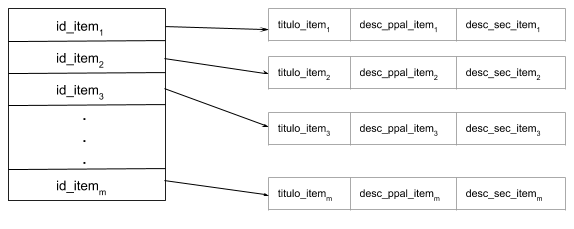
\includegraphics[width=90mm]{imagenes/estructuras/map-items.png}}
\subfigure[\scriptsize Mapa de pivotes por categor\'ias]{
\includegraphics[width=90mm]{imagenes/estructuras/categs-pivots.png}}
		\caption{\small Estructuras de datos utilizadas}
		\label{fig:estructuras}
\end{figure}

\section{Software desarrollado}

El desarrollo realizado consta de dos partes complementarias: la funcionalidad de creaci\'on de \'indices y la funcionalidad de b\'usqueda propiamente dicha, que utiliza los \'indices creados por la primera funcionalidad.\\



\subsection{Creaci\'on de \'indices para las b\'usquedas}

La funcionalidad de creaci\'on de \'indices se desarroll\'o en forma gen\'erica, preparada para recibir los siguientes par\'ametros: tipo de pivotes (random o incremental), cantidad de pivotes y conjunto de pivotes (mismo conjunto para todas las categor\'ias o diferentes conjuntos para cada categor\'ia)\\

La l\'ogica b\'asica del algoritmo de creaci\'on de \'indices carga los archivos descritos en la secci\'on  \textbf{Procesamiento inicial de los datos de entrada} en las estructuras de datos correspondientes, y procede a generar las firmas de los items, utilizando en primera instancia la estrategia de selecci\'on de pivotes en conjunci\'on con el resto de los par\'ametros (cantidad y conjunto de pivotes). Luego de completar la estructura con las firmas de los items, almacena cada estructura en un archivo de datos serializados; para que puedan ser utilizados en futuras b\'usquedas.\\

\begin{algorithm}[caption={Creaci\'on de \'indice}, label={alg1}]
crearIndice(File fCategs, File fPivs, String estSel, int cantPivs)
begin
 /* Se inicializan las estructuras */
 Hash categsHash = inicializarHashCategorias(fCategs)
 Map pivotesPorCateg
 /* Se obtiene el conjunto de pivotes en base a la estrategia */
 if(estSel == "random")
 begin
  pivotesPorCateg = obtConjPivsRandom(fPivs, cantPivs)
 end

 if(estSel == "incremental")
 begin
  pivotesPorCateg = obtConjPivsIncremental(fPivs, cantPivs)
 end

 Map items
 /*Se calculan las firmas para todos los items*/
 forall item in archivoItems
 begin
  Pivotes pivs = pivotesPorCateg.get(item.categ)
  Dist[] d = calcularDistancias(item.cod_titulo, pivotes)
  categsHash.get(item.categ).add(d)
  items.put(item.id, item)
 end
 /* Se almacenan las estructuras que componen el indice en archivos 
  * para su utilizacion futura */
 generarArchivoSerializado(categsHash)
 generarArchivoSerializado(pivotesPorCateg)
 generarArchivoSerializado(items)
end
\end{algorithm}

A continuaci\'on se presenta el pseudo-c\'odigo de los algoritmos de selecci\'on de pivotes, para facilitar la lectura de los mismos solo se incluy\'o la variante de distinto conjunto de pivotes para cada categor\'ia.

\begin{algorithm}[caption={Selecci\'on de pivotes random}, label={alg2}]
obtConjPivsRandom(File fPivs, int cantPivs)
begin
 Map conjuntoFinal
 Map pivotesPorCateg = obtenerPivotesPorCateg(fPivs)
 for(categ, pivotes in pivotesPorCateg)
 begin
  /* Se eliminan elementos random hasta alcanzar la cantidad de 
   * pivotes deseada */
  while(pivotes.size > cantPivs)
  begin
   eliminarElementoRandom(pivotes)
  end
  conjuntoFinal.put(categ, pivotes)
 end
 return conjuntoFinal
end
\end{algorithm}

\begin{algorithm}[caption={Selecci\'on de pivotes incremental}, label={alg3}]
obtConjPivsIncremental(File fPivs, int cantPivs)
begin
 Map conjuntoFinal
 Map pivotesPorCateg = obtenerPivotesPorCateg(fPivs)
 for(categ, pivotes in pivotesPorCateg)
 begin
  conjuntoPivotes
  int candidato, selec
  float dim, max
  for(i = 1 to cantPivs)
  begin
   /* Se elige un candidato inicial */ 
   selec = random(n)
   while(selec ya haya sido elegido antes)
    selec = random(n)
   conjuntoPivotes->puntos[i] = pivotes->puntos[selec]
   /* 10 es la cantidad de pares de elementos para el calculo
    * de la media D */
   max = mediaD(conjuntoPivotes, 10)
   candidato = selec
   for j = 2 to 10
    begin
    /* Se busca nuevo cantidato */
    selec = random(n)
    while(selec ya haya sido escogido antes)
     selec=random(n)
    conjuntoPivotes->puntos[i] = pivotes->puntos[selec]
    /* 10 es la cantidad de pares de elementos para el calculo 
     * de la media D */
    dim = mediaD(conjuntoPivotes, 10)
    if(dim > max)
    begin
     max = dim
     candidato = selec
    end
   end
   conjuntoPivotes->puntos[i] = pivotes->puntos[candidato]
  end
  conjuntoFinal.put(categ, pivotes)
 end
 return conjuntoFinal
end
\end{algorithm}

Como se puede inferir entonces, el algoritmo de creaci\'on de indices particiona el universo de datos $U$ (los productos) a trav\'es de las categor\'ias hojas, resultando en multiples $U_i$ listas que potencialmente contienen elementos relevantes para una consulta.\\

\subsection{Busqueda por similitud}

Se implementaron dos funcionalidades de b\'usqueda: b\'usqueda por rango, que recibe por par\'ametro el radio de b\'usqueda, la categor\'ia del producto y el t\'itulo de un producto existente; y b\'usqueda de los k-vecinos, que recibe por par\'ametro la cantidad de elementos a retornar (k), la categor\'ia del producto y el t\'itulo de un producto existente.\\

La b\'usqueda por rango calcula la distancia del t\'itulo del producto dado por par\'ametro a cada uno de los pivotes, y luego compara esa firma contra las firmas de los productos de la categor\'ia seleccionada. Este paso devuelve los productos candidatos a formar parte de la respuesta final, los cuales son utilizados para calcular la distancia real de edici\'on contra el producto buscado, descartando aquellos que est\'en fuera del rango especificado.\\

\begin{algorithm}[caption={B\'usqueda por rango}, label={alg4}]
busquedaPorRango(String q, String categ, int radio)
begin
 Pivotes pivotes = pivotesPorCateg.get(categ)
 /* Se calcula la firma para la query */
 Dist[] d = calcularDistancia(q, pivotes)
 List candidatos = []
 /* Se obtienen todas las firmas para la categoria */
 List[Dist[]] firmas = categsHash.get(categ)
 /* Se compara la firma de la query con las firmas de la categoria, 
  * si el valor es mayor que el radio, se descarta el item */
 for(j = 0 to firmas.size)
 begin
  int[] dists = firmas[j].dists
  boolean agregar = true
  for (i = 0 to dists.size)
  begin
   int value = valorAbsoluto(sig.dists[i] - dists[i])
   if (value > radio)
   begin
    i = dists.size
    agregar = false
   end
  end
  if(agregar)
   candidatos.add(firmas[j])
 end
 List itemsEncontrados = []
 for(i = 0 to candidatos.size)
 begin
  Item item = items.get(candidatos[i].id)
  int dist = distanciaEdicion(q, item.cod_titulo)
  if((radio - dist) > 0)
   itemsEncontrados.add(item)
 end
 return itemsEncontrados
end
\end{algorithm}

La b\'usqueda de los k-vecinos utiliza una variaci\'on de la b\'usqueda por rango, comenzando con un rango de 5 e incrementando ese valor hasta llegar a la cantidad deseada de resultados.\\

\begin{algorithm}[caption={B\'usqueda de los k-vecinos}, label={alg5}]
busquedaKVecinos(String q, String categ, int radio, int k)
begin
 int radio = 0
 int i = 1
 List resultadoFinal
 List itemsTemp = []
 while(itemsTemp.size < k)
 begin
  radio = potencia(5,i)
  itemsTemp = busquedaPorRango(q, categ, radio)
  /* Si se obtuvieron mas elementos que el k deseado, se procede 
   * a realizar una biseccion del radio */
  if(itemsTemp.size > k)
  begin
   int li = potencia(5,i - 1)
   int ls = radio
   /* Se realiza una biseccion del radio */
   while(li <= ls)
   begin
    radio = ((ls + li)/2)
    itemsTemp = busquedaPorRango(q, categ, radio)
    /* Se alcanzo el numero deseado de elementos, se finaliza la biseccion */
    if(itemsTemp.size == k)
    begin
     li = ls + 1
     resultadoFinal = itemsTemp
    end
    /* Se continua la biseccion para uno u otro lado, dependiendo 
     * de si se supero o no la cantidad de elementos */
    else
    begin
     if(itemsTemp.size < k)
     begin
      li = radio + 1
      radio = radio + 1
     end
     else
      ls = radio - 1
    end
   end
   if(itemsTemp.size != k)
   begin
    /* Si el ultimo resultado de la biseccion obtuvo menos elementos,
     * se debe hacer la b\'usqueda con el valor final del radio */
    if(itemsTemp.size < k)
     itemsTemp = busquedaPorRango(q, categ, radio)
    /* Se ordenan los elementos por su distancia y se seleccionan los k primeros */
    ordenarPorMenorDistancia(itemsTemp)
    resultadoFinal = itemsTemp.subList(0,k)
   end
  end
  else
   resultadoFinal = itemsTemp
  i = i + 1 
 end
 return resultadoFinal
end
\end{algorithm}

Como funcionalidad auxiliar, se implement\'o un proceso de carga que puede ser utilizado al iniciar el programa, para cargar los archivos de \'indices previamente generados.\\


\section{Re-particionado del universo}

Luego de planificar y diseñar e implementar todas las estructuras de datos, realizamos pruebas manuales para asegurarnos del correcto funcionamiento del software completo.\\

Ante \'estas pruebas, detectamos que el particionado no era sem\'anticamente correcto, ya que al elegir la categor\'ia hoja del \'arbol, estabamos restringiendo demasiado el universo de b\'usqueda. Representando la situaci\'on con un ejemplo, supongamos que deseamos recomendar productos similares al producto \textit{“Samsung Galaxy A30 32 GB Blanco 3 GB RAM”}, la categor\'ia hoja de dicho producto es \textit{“A30”}, dentro del \'arbol: \textit{“Celulares y Tel\'efonos > Celulares y Smartphones > Samsung > A30”}, si solo tenemos en cuenta los productos que pertenecen a la categor\'ia \textit{“A30”}, es probable que no encontremos, por ejemplo, celulares blancos de 32 GB de la marca Motorola.
Por \'este motivo, definimos volver a particionar el universo de productos, \'esta vez utilizando la categor\'ia inicial del \'arbol (Celulares y Tel\'efonos en el ejemplo anterior).\\

Con \'esta nueva estrategia, obtuvimos 30 particiones distintas de nuestro universo, para las cuales realizamos los experimentos descritos en el pr\'oximo cap\'itulo.
